% Figure 1, panel C artwork only.  The panel identifier and caption belong in LaTeX.
\definecolor{ink}{HTML}{1F2937}
\definecolor{muted}{HTML}{64748B}
\definecolor{rulegray}{HTML}{CBD5E1}
\definecolor{calblue}{HTML}{2563A6}
\definecolor{retainpurple}{HTML}{6B4E9B}

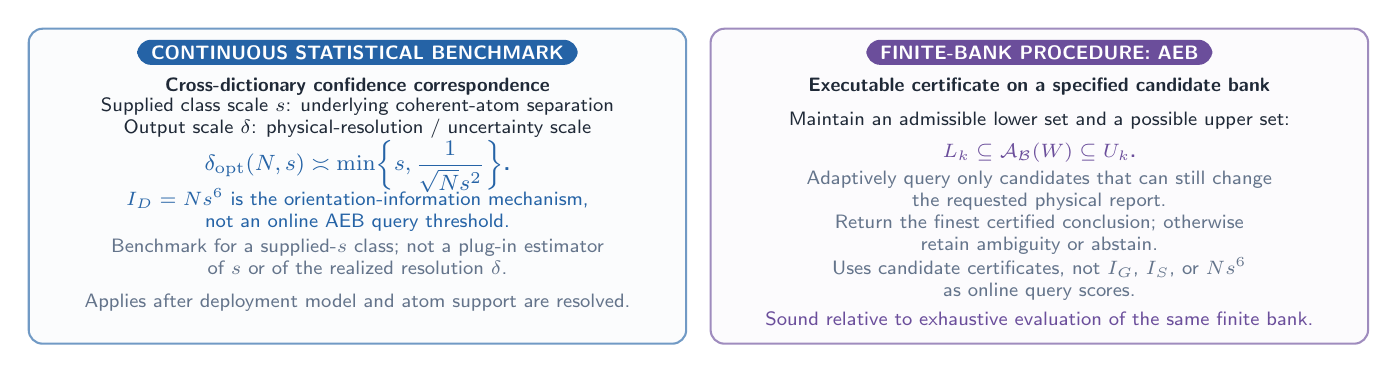
\begin{tikzpicture}[
  x=1cm,
  y=1cm,
  font=\sffamily,
  card/.style={draw=rulegray,line width=.75pt,rounded corners=5pt,fill=white},
  pill/.style={rounded corners=5pt,inner xsep=5pt,inner ysep=2.1pt,
    font=\sffamily\bfseries\scriptsize,text=white},
  resultcard/.style={card,minimum width=8.35cm,minimum height=4.00cm}
]

\begin{scope}[yshift=2.20cm]
\node[resultcard,draw=calblue!65,fill=calblue!2] (theory) at (4.42,-2.18) {};
\node[pill,fill=calblue] at ([yshift=1.70cm]theory.center)
  {CONTINUOUS STATISTICAL BENCHMARK};
\node[font=\sffamily\bfseries\scriptsize,text=ink,align=center]
  at ([yshift=1.27cm]theory.center) {Cross-dictionary confidence correspondence};
\node[font=\sffamily\scriptsize,text=ink,align=center]
  at ([yshift=.86cm]theory.center)
  {Supplied class scale $s$: underlying coherent-atom separation\\
   Output scale $\delta$: physical-resolution / uncertainty scale};
\node[font=\sffamily\bfseries\footnotesize,text=calblue]
  at ([yshift=.25cm]theory.center)
  {$\displaystyle \delta_{\mathrm{opt}}(N,s)
    \asymp \min\!\left\{s,\frac{1}{\sqrt{N}s^2}\right\}$.};
\node[font=\sffamily\scriptsize,text=calblue,align=center]
  at ([yshift=-.30cm]theory.center)
  {$I_D=Ns^6$ is the orientation-information mechanism,\\
   not an online AEB query threshold.};
\node[font=\sffamily\scriptsize,text=muted,align=center]
  at ([yshift=-.90cm]theory.center)
  {Benchmark for a supplied-$s$ class; not a plug-in estimator\\
   of $s$ or of the realized resolution $\delta$.};
\node[font=\sffamily\scriptsize,text=muted,align=center]
  at ([yshift=-1.48cm]theory.center)
  {Applies after deployment model and atom support are resolved.};

\node[resultcard,draw=retainpurple!65,fill=retainpurple!2]
  (aeb) at (13.08,-2.18) {};
\node[pill,fill=retainpurple] at ([yshift=1.70cm]aeb.center)
  {FINITE-BANK PROCEDURE: AEB};
\node[font=\sffamily\bfseries\scriptsize,text=ink,align=center]
  at ([yshift=1.27cm]aeb.center)
  {Executable certificate on a specified candidate bank};
\node[font=\sffamily\scriptsize,text=ink,align=center]
  at ([yshift=.83cm]aeb.center)
  {Maintain an admissible lower set and a possible upper set:};
\node[font=\sffamily\bfseries\scriptsize,text=retainpurple]
  at ([yshift=.42cm]aeb.center)
  {$L_k\subseteq\mathcal A_{\mathcal B}(W)\subseteq U_k$.};
\node[font=\sffamily\scriptsize,text=muted,align=center]
  at ([yshift=-.06cm]aeb.center)
  {Adaptively query only candidates that can still change\\
   the requested physical report.};
\node[font=\sffamily\scriptsize,text=muted,align=center]
  at ([yshift=-.62cm]aeb.center)
  {Return the finest certified conclusion; otherwise\\
   retain ambiguity or abstain.};
\node[font=\sffamily\scriptsize,text=muted,align=center]
  at ([yshift=-1.18cm]aeb.center)
  {Uses candidate certificates, not $I_G$, $I_S$, or $Ns^6$\\
   as online query scores.};
\node[font=\sffamily\scriptsize,text=retainpurple,align=center]
  at ([yshift=-1.68cm]aeb.center)
  {Sound relative to exhaustive evaluation of the same finite bank.};
\end{scope}
\end{tikzpicture}

